\documentclass{article}
\usepackage{neurips_2025}

\usepackage[utf8]{inputenc} % allow utf-8 input
\usepackage[T1]{fontenc}    % use 8-bit T1 fonts
\usepackage{hyperref}       % hyperlinks
\usepackage{url}            % simple URL typesetting
\usepackage{booktabs}       % professional-quality tables
\usepackage{amsfonts}       % blackboard math symbols
\usepackage{nicefrac}       % compact symbols for 1/2, etc.
\usepackage{microtype}      % microtypography
\usepackage{xcolor}         % colors

%privately included
\usepackage{tikz}
\usepackage{float} 
\usetikzlibrary{arrows.meta, positioning}
\usepackage{amsmath}    
\usepackage{amsfonts} 
\usepackage{amssymb}    
\usepackage{listings}
\usepackage{xcolor}

\lstset{
  language=Python,
  basicstyle=\ttfamily\small,
  keywordstyle=\color{blue},
  commentstyle=\color{gray},
  stringstyle=\color{orange},
  showstringspaces=false,
  breaklines=true,
  frame=single,
  tabsize=2
}

\title{Operand Selective Logic Gate Network}

\author{%
  Soon Ho~Choi\\
  Department of Computer Science\\
  Kookmin University\\
  Gyeonggi-do, 13629, Rep. of KOREA \\
  \texttt{sosaror@gmail.com} \\
  % examples of more authors
  % \And
  % Coauthor \\
  % Affiliation \\
  % Address \\
  % \texttt{email} \\
  % \AND
  % Coauthor \\
  % Affiliation \\
  % Address \\
  % \texttt{email} \\
  % \And
  % Coauthor \\
  % Affiliation \\
  % Address \\
  % \texttt{email} \\
  % \And
  % Coauthor \\
  % Affiliation \\
  % Address \\
  % \texttt{email} \\
}

\begin{document}
\maketitle

\begin{abstract}
We propose Operand-Selective Logic Gate Networks (OSLGN), a symbolic neural architecture that builds differentiable logic circuits via operand and operator selection. Each logic unit dynamically selects two operands from the input and applies one of sixteen predefined binary logic operators, thereby forming a symbolic computation structure that remains trainable through gradient descent. Our operator selection builds upon prior work on differentiable logic gates, while our introduction of operand selection constitutes a novel modular extension. To encourage locally coherent logic formation, we initialize operand selectors with a proximity-based prior inspired by small-world network topology. Specifically, each operand selector is biased toward selecting neighboring input features, allowing the network to efficiently compose local structures and gradually learn long-range dependencies. Experiments on MNIST demonstrate that this initialization improves generalization and stabilizes gradient flow, and we further show that despite modest classification performance, the trained network can be fully converted into compact symbolic logic expressions.
\end{abstract}


\section{Introduction}
  Neural networks have achieved remarkable success across a wide range of tasks, yet their internal representations are often entangled and difficult to modularize. While neural-symbolic reasoning and differentiable logic circuits have made progress toward combining symbolic structure with trainability~\cite{petersen2022deep, manhaeve2018deepproblog}, most architectures still struggle to express logic-based computation in a compositional and scalable way.

In this work, we introduce \textit{Operand Selective Logic Gated Networks (OSLGN)}, a symbolic neural architecture where each layer is a collection of binary logic gates. Each gate selects two operands from the previous layer via a differentiable $\arg\max$ mechanism (using a straight-through estimator), and applies one of 16 predefined binary logic operations (e.g., AND, OR, XOR). While prior works have focused on differentiable operator selection~\cite{petersen2022deep}, our key contribution is to enable operand-level routing. This allows each gate to learn not only what operation to apply, but also which inputs to apply it to—forming discrete, modular logic circuits.

To encourage the emergence of localized symbolic structure, we initialize operand selectors with a Gaussian proximity bias inspired by small-world connectivity~\cite{watts1998collective, javaheripi2019swnet}. This inductive prior promotes compositional logic among nearby nodes while still allowing long-range dependencies to emerge through learning.

We further interpret our architecture as a fine-grained form of Mixture-of-Experts~\cite{shazeer2017outrageously}, where selection happens at the operand level within each logic gate. This facilitates sparse symbolic computation with minimal overhead.

\paragraph{Contributions.}
\begin{itemize}
    \item We propose Operand-Selective Logic Gated Networks (OSLGN), a symbolic neural architecture that builds differentiable logic circuits via operand and operator selection.
    
    \item We introduce an operand selection mechanism that enables gate-level modularity. While our operator routing builds on prior differentiable logic gates~\cite{petersen2022deep}, operand selection is independently learned and crucial for symbolic structure.
    
    \item We incorporate a proximity-biased operand initialization scheme inspired by small-world networks, promoting symbolic locality and stable training dynamics.
    
    \item We show that OSLGN can be fully translated into compact logic expressions post-training, demonstrating the feasibility of distilling a neural network into an explicit symbolic circuit.
\end{itemize}

\section{OSLGN Architecture}
  \subsection{Overview}
    Operand Selective Logic Gated Neural Network (OSLGN) is a modular architecture that performs binary logic operations between selected operand features using a learned differentiable selection mechanism. The core design of OSLGN mimics the structure of a logical expression tree, where each logic unit (or layer) selects two operands from the input feature space and applies a logic gate to compute the output.

Each OSLGN layer consists of three components: two operand selectors and one operator selector. The operand selectors learn to identify and extract the most relevant features from the input by applying a sparse one-hot mask generated via an argmax operation over linear projections, smoothed using the straight-through estimator (STE) to maintain differentiability. These selectors ensure that the network can choose which elements of the input vector should interact logically at each step.

The selected operands are then passed to the operator module, which computes a binary logic operation between them. Instead of hardcoding a specific logic gate, the operator is learned as a selection over a set of 16 predefined binary logic functions (e.g., AND, OR, XOR, NAND, etc.). Unlike softmax method from petersen's research\cite{petersen2022deep} an argmax-based weighting is applied to the outputs of all gates, followed by binarization through a custom STE, allowing the model to learn with consisting logic gate identity.

By stacking multiple OSLGN layers, the architecture is able to represent hierarchical logic computations, while maintaining symbolic nature. Unlike standard neural networks, which rely on additive and multiplicative transformations, OSLGN explicitly builds logical reasoning paths via structured operand and operator selection.

\begin{figure}[H]
    \centering
    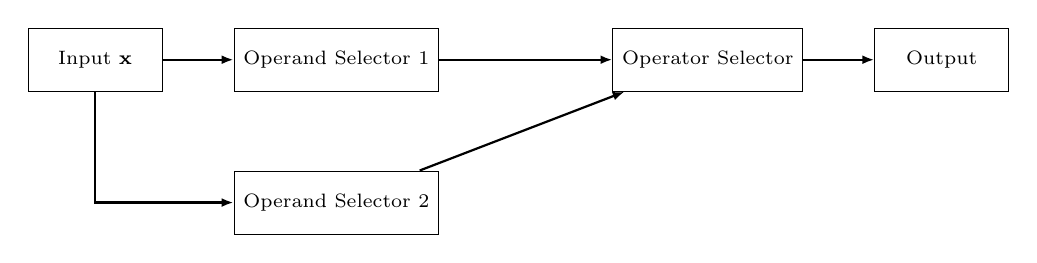
\begin{tikzpicture}[
      node distance=1cm and 0.9cm,
      every node/.style={draw, minimum width=1.7cm, minimum height=0.8cm, font=\scriptsize, align=center},
      arrow/.style={-{Latex[length=1.5mm]}, thick}
    ]
        \node (input) {Input $\mathbf{x}$};
        \node (os1) [right=of input] {Operand Selector 1};
        \node (os2) [below=of os1] {Operand Selector 2};
        \node (op) [right=2.2cm of os1] {Operator Selector};
        \node (out) [right=of op] {Output};

        \draw[arrow] (input) -- (os1);
        \draw[arrow] (input) |- (os2);
        \draw[arrow] (os1) -- (op);
        \draw[arrow] (os2) -- (op);
        \draw[arrow] (op) -- (out);
    \end{tikzpicture}
    \caption{
    A single OSLGN logic unit. Operand selectors choose relevant inputs, and a differentiable operator module applies one of 16 logic gates.
    }
    \label{fig:oslgn-block}
    \end{figure}
    
To improve training stability and promote locally coherent symbolic structures, we initialize the operand selectors using a Gaussian neighborhood prior inspired by small-world network topology~\cite{watts1998collective, javaheripi2019swnet}. This bias encourages each selector to initially focus on spatially adjacent input features, facilitating modular logic formation while allowing long-range dependencies to emerge via learning.


    
  \subsection{Operand Selection}
    In each OSLGN layer, the operand selection modules are responsible for choosing two input subcomponents from the feature vector $\mathbf{x} \in \mathbb{R}^d$ that will participate in a logical operation. We refer to these modules as Operand Selector 1 (OS1) and Operand Selector 2 (OS2). Each selector computes a linear projection over the input and applies a hard selection via the \texttt{argmax} function, followed by a one-hot masking operation.

Since \texttt{argmax} is non-differentiable, we apply the straight-through estimator (STE) to allow gradient flow during training. Specifically, we subtract the detached projection from the one-hot mask and add back the original projection, enabling gradients to flow through the selected path while preserving the discrete behavior in the forward pass:
\[
\tilde{w} = \text{onehot}(\arg\max(w)) - w.detach() + w
\]
where $w$ denotes the linear projection weights.

This masked weight vector is then used in a standard linear transformation:
\[
\mathbf{a} = \tilde{w} \cdot \mathbf{x}
\]
The same mechanism is applied to both operand selectors (OS1 and OS2), producing two selected values $\mathbf{a}$ and $\mathbf{b}$ which are subsequently passed to the operator module.

\begin{figure}[H]
    \centering
    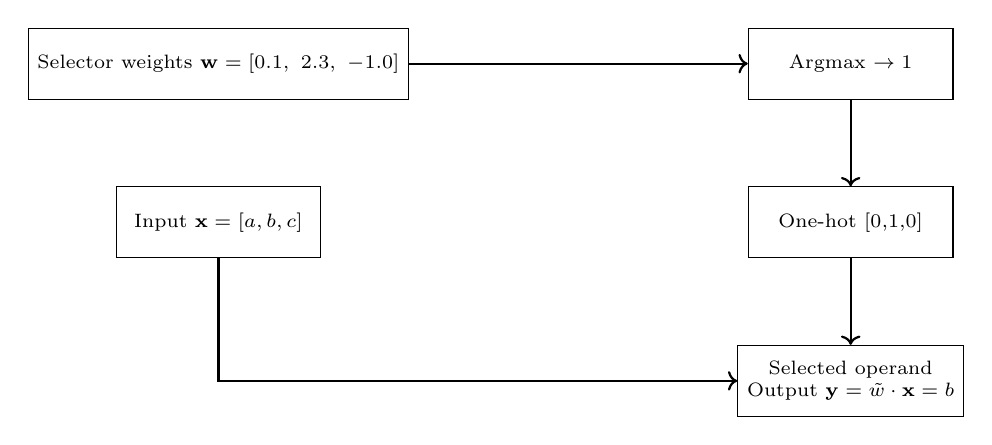
\begin{tikzpicture}[
      node distance=1.1cm and 1.5cm,
      every node/.style={draw, font=\scriptsize, minimum width=2.6cm, minimum height=0.9cm, align=center},
      arrow/.style={->, thick}
    ]
    
    \node (w) {Selector weights $\mathbf{w} = [0.1,\ 2.3,\ -1.0]$};
    \node (x) [below=of w] {Input $\mathbf{x} = [a, b, c]$};
    
    \node (argmax) [right=of w, xshift=2.8cm] {Argmax $\rightarrow 1$};
    \node (onehot) [below=of argmax] {One-hot $[0,\!1,\!0]$};
    
    \node (select) [below=of onehot] {Selected operand \\ Output $\mathbf{y} = \tilde{w} \cdot \mathbf{x} = b$};
    
    \draw[arrow] (w) -- (argmax);
    \draw[arrow] (argmax) -- (onehot);
    \draw[arrow] (onehot) -- (select);
    \draw[arrow] (x) |- (select);
    
    \end{tikzpicture}
    \caption{
    Operand selection with STE. The model uses learnable selector weights $\mathbf{w}$ to generate a one-hot mask that selects a single operand from the binary input $\mathbf{x}$ via a differentiable masking mechanism.
    }
    \label{fig:operand-selection-ste}
\end{figure}

To promote locally structured operand selection, we initialize the selector weights $\mathbf{w}$ using a Gaussian prior centered around each output index. Specifically, for the $i$-th row of OS1 and OS2, the weights are initialized as
\[
w_{ij} = \exp\left( -\frac{(j - c_i)^2}{2\sigma^2} \right), \quad c_i = (i + s) \bmod d
\]
where $d$ is the input dimension, $s$ is a small center shift (e.g., $s=0$ for OS1, $s=1$ for OS2), and $\sigma$ controls the locality. This initialization introduces a topological bias similar to small-world networks~\cite{watts1998collective}, favoring local operand pairing early in training.

  \subsection{Operation Selection}
    While Petersen et al.~\cite{petersen2022deep} utilize continuous gate weighting and perform post-hoc logic gate substitution after training, our approach incorporates a straight-through estimator (STE) mechanism that enforces discrete operator selection during training. This results in a train-time quantization effect, where symbolic logic structures are formed during optimization rather than approximated retrospectively.

Specifically, we use a hard one-hot mask over the operator logits with gradient-preserving relaxation:
\[
\tilde{\pi} = \text{onehot}(\arg\max(w)) - \text{detach}(w) + w
\]
which yields a discrete gate selection in the forward pass, while enabling gradient-based optimization. This tight coupling between learning and logical structure avoids potential mismatch between continuous representations and their final symbolic form.

\section{Related Work}
  \subsection{Logic Neural Networks and Symbolic Computation}
    Neural-symbolic models aim to integrate logical reasoning into neural networks. Early efforts like DeepProbLog~\cite{manhaeve2018deepproblog} and Logic Tensor Networks~\cite{serafini2016logic} incorporated symbolic logic via probabilistic inference or fuzzy semantics, but required predefined logic templates. Neural Logic Machines~\cite{dong2019nlm} introduced trainable logical operations, yet imposed rigid operand structures.

Logical Neural Networks (LNNs)~\cite{riegel2020lnn} extended this line by learning differentiable representations of logical formulas using fuzzy logic operators at the neuron level. While expressive, their logic is embedded in continuous-valued activations. In contrast, our model composes discrete logic circuits via operand and operator selection, allowing symbolic structure to emerge during training. This enables our system to approximate logic expressions in a form directly symbolizable.

  \subsection{Mixture-of-Experts and Modular Routing}
    Mixture-of-Experts (MoE) architectures enable conditional computation by activating only a subset of experts per input, enhancing scalability and efficiency. Pioneering works like the Sparsely-Gated MoE~\cite{shazeer2017outrageously} and Switch Transformer~\cite{fedus2022switch} utilize token-level top-k routing. Expert Choice Routing~\cite{zhou2022mixture} reverses this paradigm, allowing experts to select tokens, improving load balancing.

Recent advancements introduce fine-grained routing and sparse masking techniques. DSelect-k~\cite{hazimeh2021dselect} offers differentiable top-k selection without softmax, while BASE Layers~\cite{lewis2021base} employ linear assignment for expert allocation, mitigating expert collapse. Hash Layers~\cite{roller2021hash} provide deterministic routing via hashing functions, eliminating the need for learned gating.

Our approach diverges by implementing operand and operator-level routing within logic gate modules, utilizing argmax with Straight-Through Estimator (STE) for discrete selection. This fine-grained, symbolic routing contrasts with traditional MoE strategies, enabling the construction of symbolic logic circuits within neural networks.

  \subsection{Discrete Selection and Straight-Through Estimators}
    Training neural networks with discrete operations poses challenges due to non-differentiability. The Straight-Through Estimator (STE)~\cite{bengio2013estimating} addresses this by treating discrete operations as identity functions during backpropagation, enabling gradient flow through non-differentiable units.

The Gumbel-Softmax trick~\cite{jang2016categorical, maddison2016concrete} offers a continuous relaxation of categorical distributions, allowing differentiable sampling. Combining STE with Gumbel-Softmax, the Straight-Through Gumbel-Softmax (ST-GS) estimator performs discrete sampling in the forward pass and uses the relaxed distribution for gradient computation in the backward pass.

Recent advancements, such as Decoupled ST-GS~\cite{shah2024improving}, introduce separate temperature parameters for forward and backward passes, enhancing gradient fidelity and training stability.

In our work, we employ argmax-based discrete selection with STE for operand and operator routing within logic gates. This approach ensures the construction of symbolizable logic circuits. While Gumbel-Softmax-based methods demonstrated faster convergence in preliminary experiments, they exhibited instability in training dynamics. Future work may explore integrating advanced techniques like Decoupled ST-GS to balance convergence speed and training stability.

  \subsection{Topological Structures in Deep Learning}
    We investigate how incorporating local topological priors into operand selection affects training dynamics and generalization. Inspired by the locality structure of small-world networks~\cite{watts1998collective}, we initialize each operand selector (\texttt{os1}, \texttt{os2}) to prefer inputs that are spatially adjacent. Specifically, the $i$-th output of \texttt{os1} is initialized to select around input index $i$, while \texttt{os2} is initialized around $i+1$, using a circular Gaussian kernel. No long-range connectivity is imposed; such dependencies must emerge via learning.

We compare this inductive bias (\textit{local init}) with standard dense initialization (\textit{no init}) using OSLGN models with depth 4 and width 512 on MNIST. All other configurations (loss, optimizer, batch size) are held constant.

\paragraph{Generalization.}
As shown in Figure~\ref{fig:smallworld_acc}, the model with local operand initialization achieves higher validation accuracy (39.9\%) compared to standard initialization (34.9\%), despite having lower training accuracy. This suggests that early locality constraints serve as a useful regularizer for symbolic composition.

\paragraph{Gradient Dynamics.}
We further observe that local init results in lower and more stable layer-wise gradient norms (Figure~\ref{fig:smallworld_gradnorm}). This implies that operand selection in the early training phase is smoother and more modular, avoiding large gradient spikes often caused by arbitrary operand mixing.

\paragraph{Learned Distant Connection.}
Although no explicit small-world graph is instantiated, our design encourages a functional small-world effect: high local clustering (via neighborhood initialization) and potential for long-range connections (via training). This stands in contrast to graph-based small-world CNNs~\cite{javaheripi2019swnet}, where topology is hard-coded rather than learned.
The full code used to reproduce these experiments is available at: \footnote{\url{https://colab.research.google.com/drive/1iJpgwW6_7oRRcbllWPLOIW9eeZ0Hcwce?usp=sharing}}

\begin{figure}[H]
    \centering
    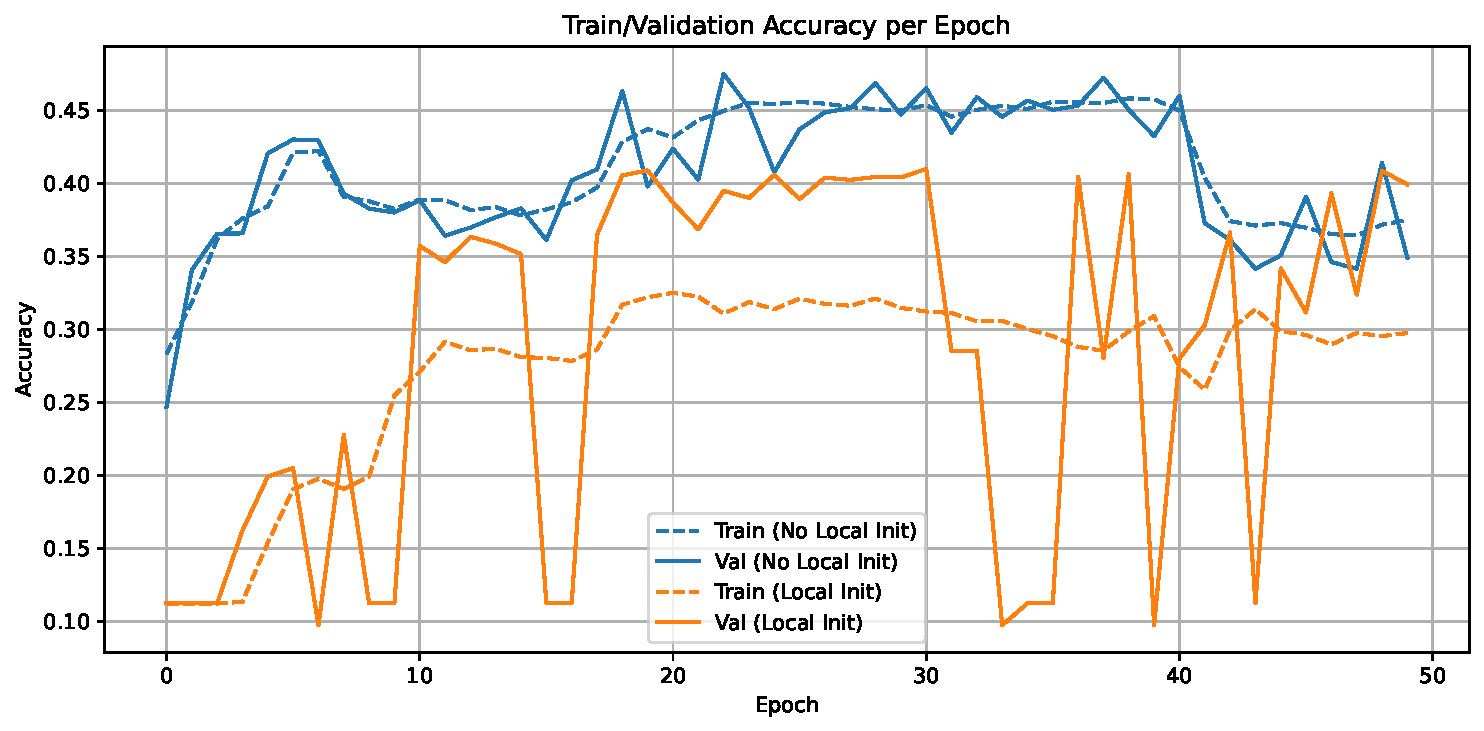
\includegraphics[width=0.45\textwidth]{figures/small_world/accuracy.pdf}
    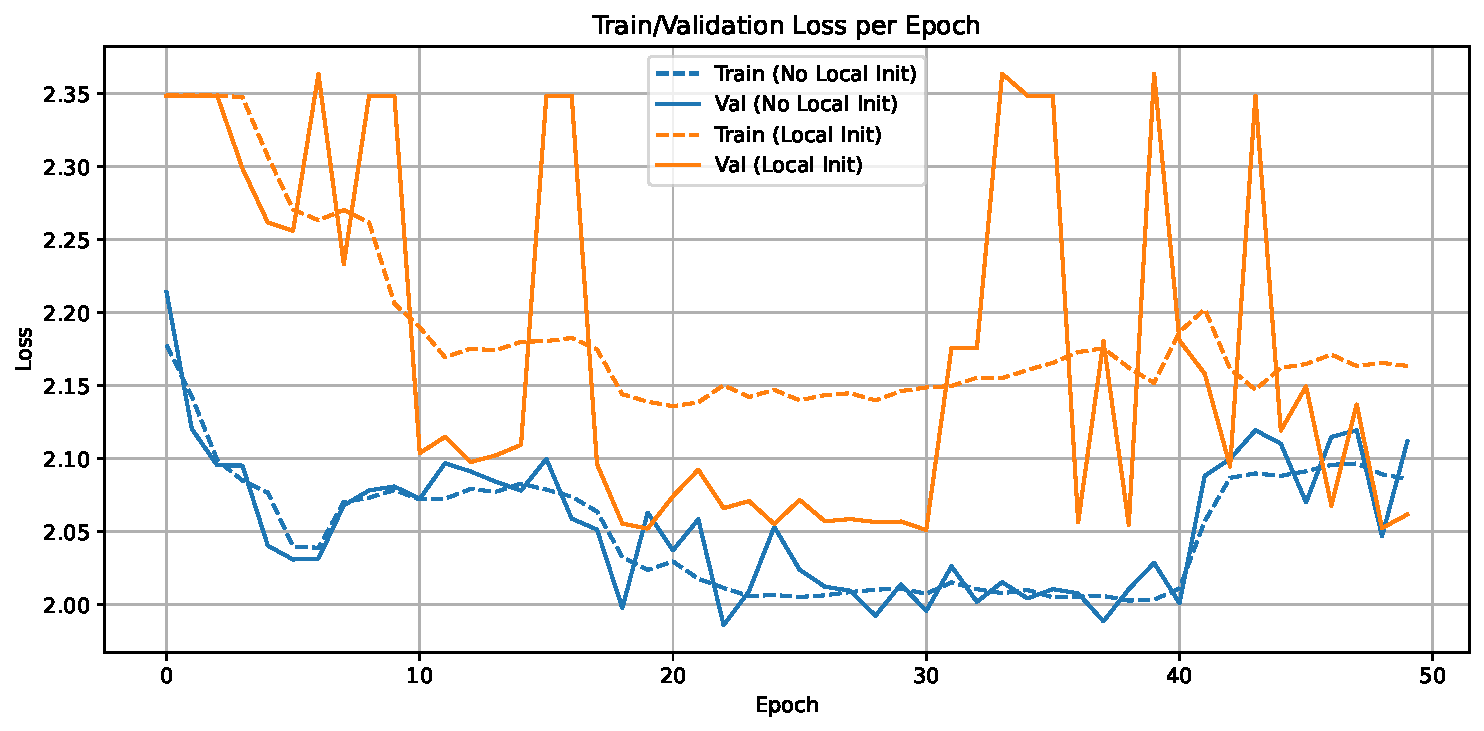
\includegraphics[width=0.45\textwidth]{figures/small_world/loss.pdf}
    \caption{Training and validation accuracy/loss over epochs for OSLGN with and without local operand initialization. Local init generalizes better.}
    \label{fig:smallworld_acc}
\end{figure}

\begin{figure}[H]
    \centering
    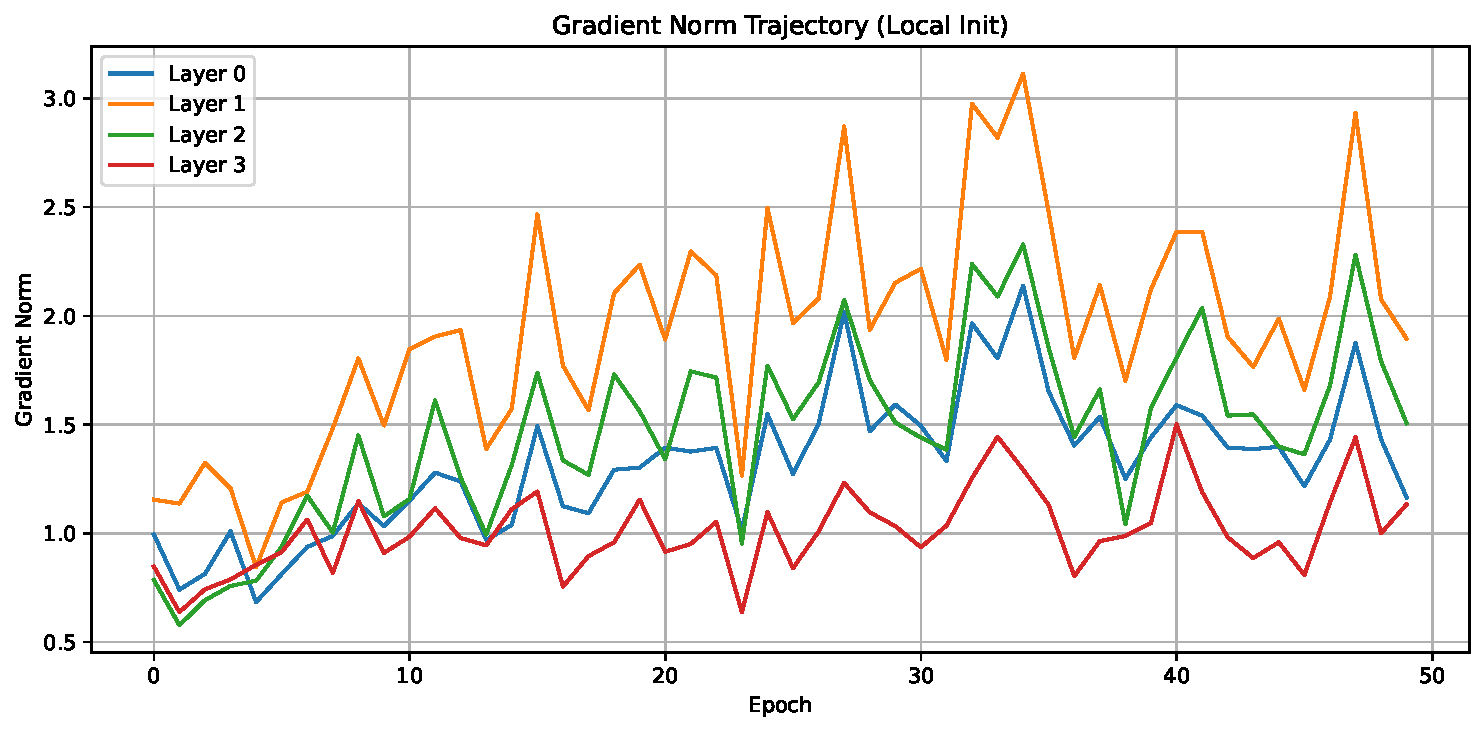
\includegraphics[width=0.85\textwidth]{figures/small_world/gradnorm_lineplot_localinit_on.pdf} \\
    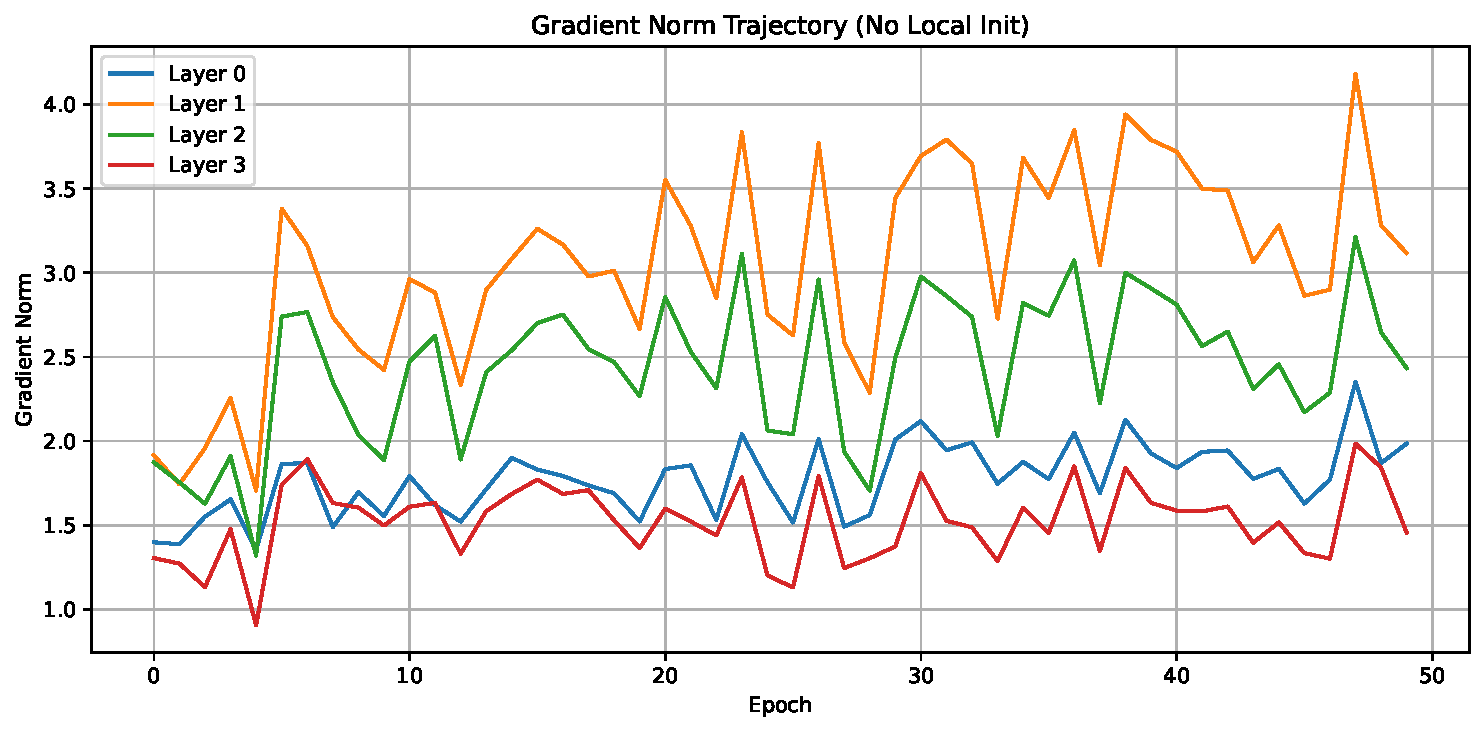
\includegraphics[width=0.85\textwidth]{figures/small_world/gradnorm_lineplot_localinit_off.pdf}
    \caption{Layer-wise gradient norm trajectories with (top) and without (bottom) local operand initialization. Local init results in smoother gradient flow.}
    \label{fig:smallworld_gradnorm}
\end{figure}


\section{Experiments}\label{sec:experiments}
    Experiments are performed in google colab. Every ipynb is shared via link. MNIST\cite{deng2012mnist} dataset is used.
  \subsection{Ablation Study: Operand Gradient Detachment}
    To assess the importance of gradient flow through operand selection, we compare two variants of the OSLGN model that share identical architectures but differ in how operands contribute to learning:

\begin{itemize}
    \item \textbf{Model A (STE-enabled)}: Operands are selected using an $\arg\max$ mask with straight-through estimation, enabling gradients to update operand selectors.
    \item \textbf{Model B (Detached)}: The outputs of operand selectors are detached from the computation graph, preventing any gradient flow into operand selection.
\end{itemize}

Both models were trained on binarized MNIST using the same initialization, optimizer, and training schedule.  
Table~\ref{tab:operand-detach-results} shows that Model A achieves significantly higher performance, reaching a test accuracy of 42.2\% compared to just 8.9\% for Model B.  
This suggests that operand selection must remain differentiable for the network to learn meaningful logic compositions.

To ensure logical validity, all outputs of the logic gate layer were enforced to be strictly binary (\texttt{0} or \texttt{1}) using runtime assertions during training.  
The full training script and model code are publicly available via Colab\footnote{\url{https://colab.research.google.com/drive/1ykNB-ezkUh9NhR1eGCZwtzsapPIp_BtM}}, and a complete implementation of the model is included in Appendix~\ref{appendix:model-code}.

\begin{table}[H]
    \caption{Operand gradient ablation: detaching operand selection leads to poor performance, confirming its critical role in learning.}
    \label{tab:operand-detach-results}
    \centering
    \begin{tabular}{lcc}
        \toprule
        \textbf{Model} & \textbf{Train Accuracy} & \textbf{Test Accuracy} \\
        \midrule
        Model A (STE-enabled) & 43.3\% & 42.2\% \\
        Model B (Detached)    & 10.0\% & 8.9\% \\
        \bottomrule
    \end{tabular}

\end{table}

  \subsection{Depth Scaling}\label{subsec:Depth Scaling}
    We investigate how the OSLGN architecture scales with network depth by evaluating variants with 2, 4, and 8 stacked logic layers, each composed of operand and operator selection modules. 
All models are trained for 50 epochs on MNIST with identical hyperparameters.

Figure~\ref{fig:accuracy} shows that the depth-8 model achieves the highest validation accuracy across all depths, slightly outperforming the depth-4 variant. 
However, the depth-4 model converges more steadily and reaches its peak accuracy earlier, while the depth-8 model continues to improve but with higher variance. 
The depth-2 model converges quickly but saturates early. 
These results suggest that deeper OSLGN networks can achieve higher performance, but require more training and exhibit less stability during convergence.

\begin{figure}[H]
    \centering
    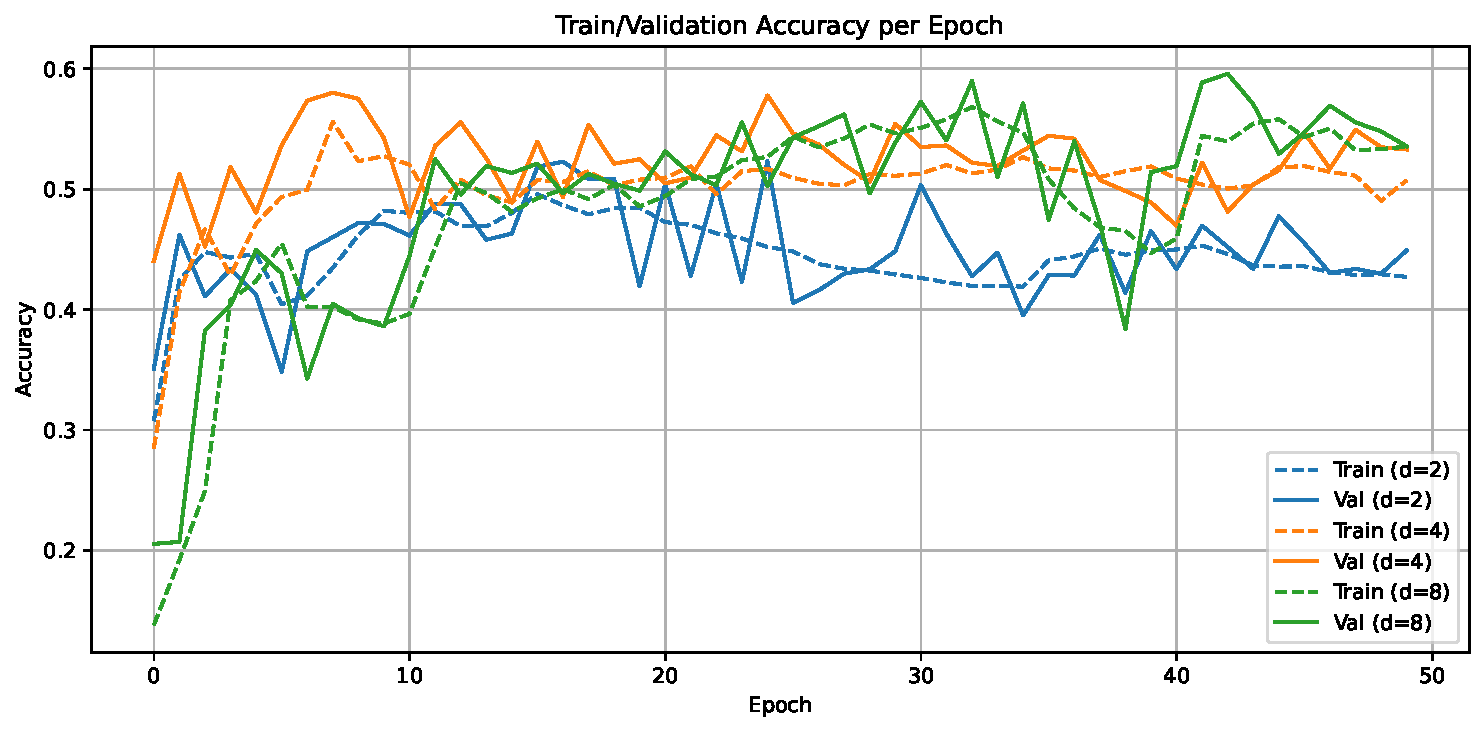
\includegraphics[width=0.85\linewidth]{figures/accuracy.pdf}
    \caption{Train and validation accuracy across 50 epochs for OSLGN models of varying depth. Depth-8 achieves the highest validation accuracy, but depth-4 shows more stable convergence.}
    \label{fig:accuracy}
\end{figure}

\begin{figure}[H]
    \centering
    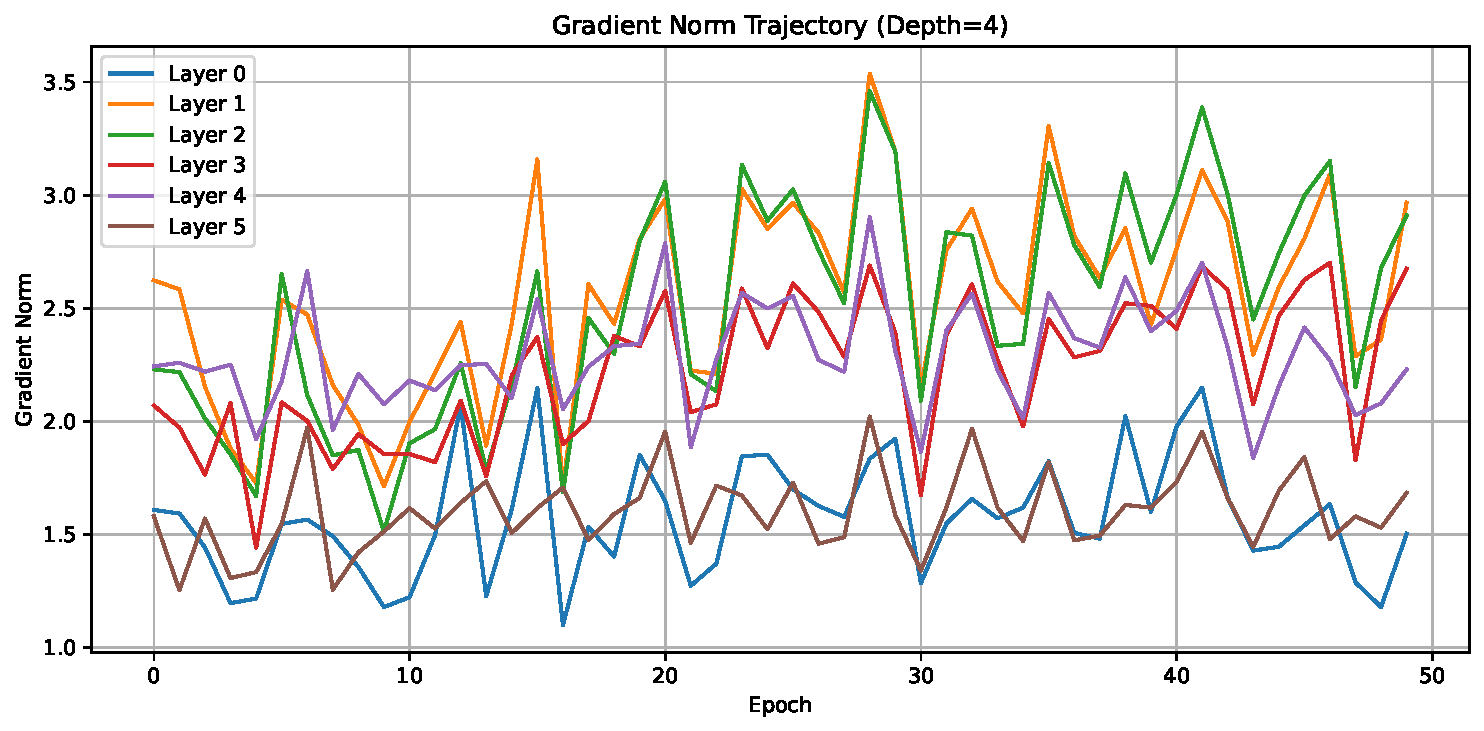
\includegraphics[width=0.45\linewidth]{figures/gradnorm_lineplot_depth4.pdf}
    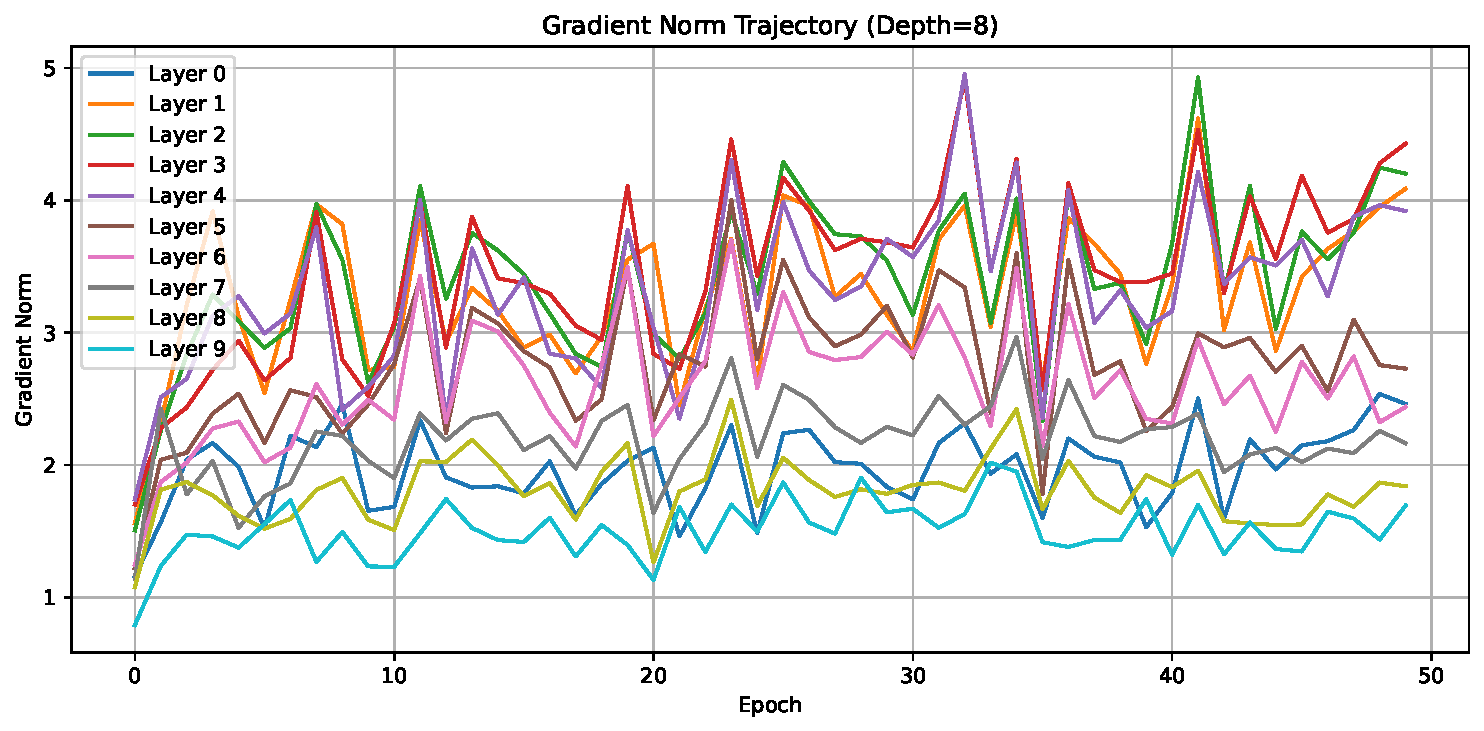
\includegraphics[width=0.45\linewidth]{figures/gradnorm_lineplot_depth8.pdf}
    \caption{Gradient norm per layer in depth-4(left) and depth-8(right) model. Optimization of depth 8 is less stable, and layer-wise imbalance is more prominent.}
    \label{fig:gradnorm_line_depth4}
\end{figure}

Figure~\ref{fig:gradnorm_line_depth4} show per-layer gradient norms for depth-4 and depth-8 models, respectively. 
We observe no gradient vanishing across layers; however, the depth-8 model exhibits more pronounced fluctuations and greater disparity between layers, suggesting optimization imbalance in deeper compositions.

Unlike conventional architectures, OSLGN does not employ normalization layers or residual connections, as these mechanisms interfere with the discrete and symbolic structure of binary logic gates. 
This design choice preserves the model’s logic circuit equivalence, but it also introduces training challenges, particularly in deeper networks.

Our implementation\footnote{\url{https://colab.research.google.com/drive/1PZhAzfH9bh_2cVn3s_Clmgkj0ezVr3Jw}} is publicly available and supports configurable depth, logging, and visualization, allowing researchers to explore the scalability of logic-based neural circuits further.

  \subsection{Logic Symbol Compression}
    To evaluate the symbolic expressiveness and compressibility of OSLGN, we extract discrete Boolean expressions from trained models and analyze their logical redundancy. This process is made possible by the discrete nature of the architecture: each layer consists of a set of binary logic gates whose operand and operator selections are recorded during training.

Following training, each class-specific computation path is reconstructed as a Boolean expression using recursive backtracking from the final output node to input variables. These expressions use only \texttt{and}, \texttt{or}, and \texttt{not} operators, forming a fully symbolic circuit.

We apply logic minimization using the \texttt{pyeda.boolalg.espresso} package~\cite{piazza2014pyeda}, which internally interfaces with the well-known \textsc{Espresso} algorithm~\cite{brayton1984espresso} for two-level Boolean minimization. For each class expression, we compare the number of logic operators before and after simplification to assess compressibility.

\vspace{0.5em}
\noindent \textbf{Example: Class 0}

\begin{quote}
\begin{verbatim}
[Original]
((((not (x[462] or x[407]) and (x[482] or x[484]))) and 
not ((False) and not ((x[578] or not x[363]) or not (x[107])))) or (False))

[Compressed]
((not x[462] and not x[407] and x[482]) or (not x[462] and 
not x[407] and x[484]))
\end{verbatim}
\end{quote}

While the compressed form often increases in length, this is due to disjunctive normal form (DNF) expansion that enumerates input conditions explicitly~\cite{sipser2012introduction}. The native OSLGN representation is already compact, demonstrating its structural efficiency.

\vspace{0.5em}
The remaining expressions, along with full source code and symbolic reconstruction routines, are provided in Appendix~\ref{appendix:symbolic} and available at our public Colab notebook:\footnote{\url{https://colab.research.google.com/drive/1VxulftRzLRj1Yg6C-vhmfE6X5jJpxfwJ}}

  \subsection{Effect of Local Operand Initialization}
    We investigate how incorporating local topological priors into operand selection affects training dynamics and generalization. Inspired by the locality structure of small-world networks~\cite{watts1998collective}, we initialize each operand selector (\texttt{os1}, \texttt{os2}) to prefer inputs that are spatially adjacent. Specifically, the $i$-th output of \texttt{os1} is initialized to select around input index $i$, while \texttt{os2} is initialized around $i+1$, using a circular Gaussian kernel. No long-range connectivity is imposed; such dependencies must emerge via learning.

We compare this inductive bias (\textit{local init}) with standard dense initialization (\textit{no init}) using OSLGN models with depth 4 and width 512 on MNIST. All other configurations (loss, optimizer, batch size) are held constant.

\paragraph{Generalization.}
As shown in Figure~\ref{fig:smallworld_acc}, the model with local operand initialization achieves higher validation accuracy (39.9\%) compared to standard initialization (34.9\%), despite having lower training accuracy. This suggests that early locality constraints serve as a useful regularizer for symbolic composition.

\paragraph{Gradient Dynamics.}
We further observe that local init results in lower and more stable layer-wise gradient norms (Figure~\ref{fig:smallworld_gradnorm}). This implies that operand selection in the early training phase is smoother and more modular, avoiding large gradient spikes often caused by arbitrary operand mixing.

\paragraph{Learned Distant Connection.}
Although no explicit small-world graph is instantiated, our design encourages a functional small-world effect: high local clustering (via neighborhood initialization) and potential for long-range connections (via training). This stands in contrast to graph-based small-world CNNs~\cite{javaheripi2019swnet}, where topology is hard-coded rather than learned.
The full code used to reproduce these experiments is available at: \footnote{\url{https://colab.research.google.com/drive/1iJpgwW6_7oRRcbllWPLOIW9eeZ0Hcwce?usp=sharing}}

\begin{figure}[H]
    \centering
    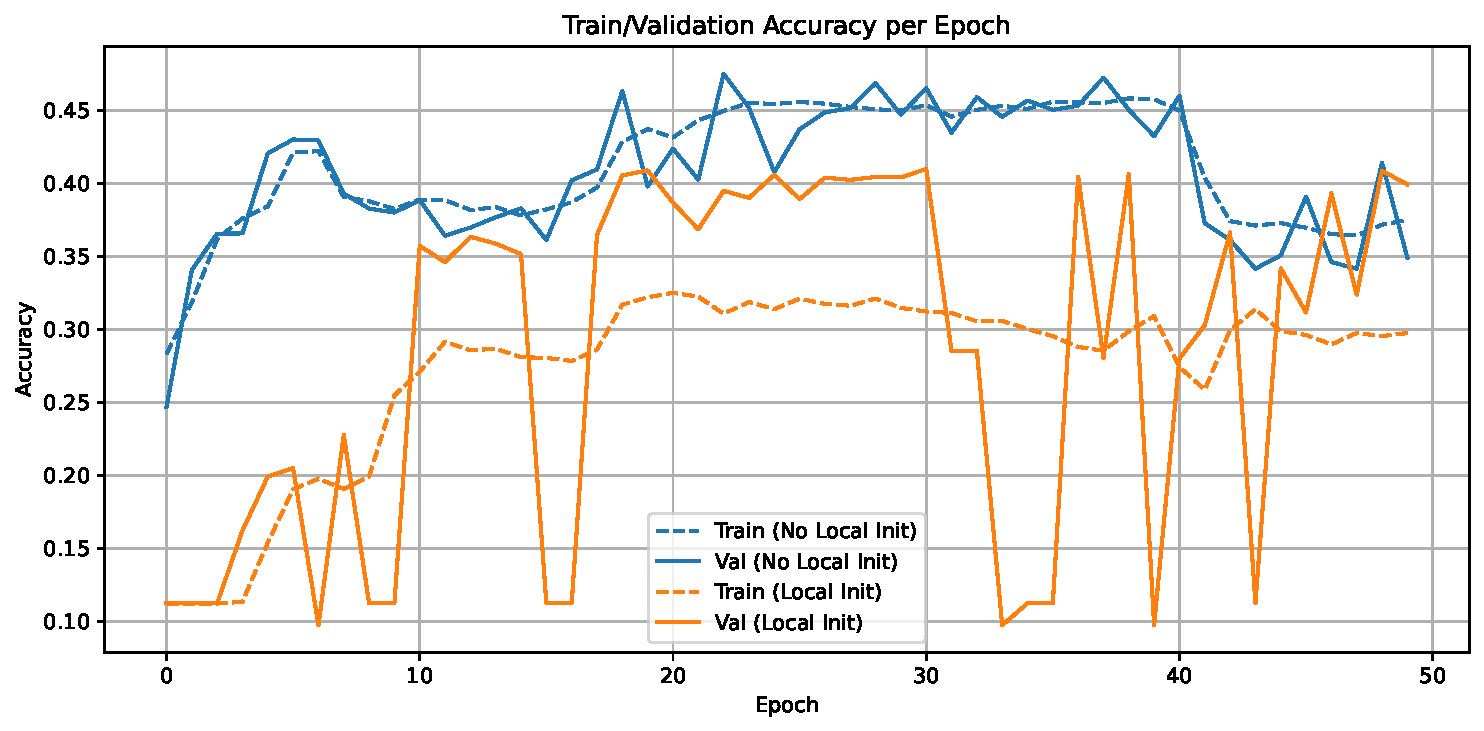
\includegraphics[width=0.45\textwidth]{figures/small_world/accuracy.pdf}
    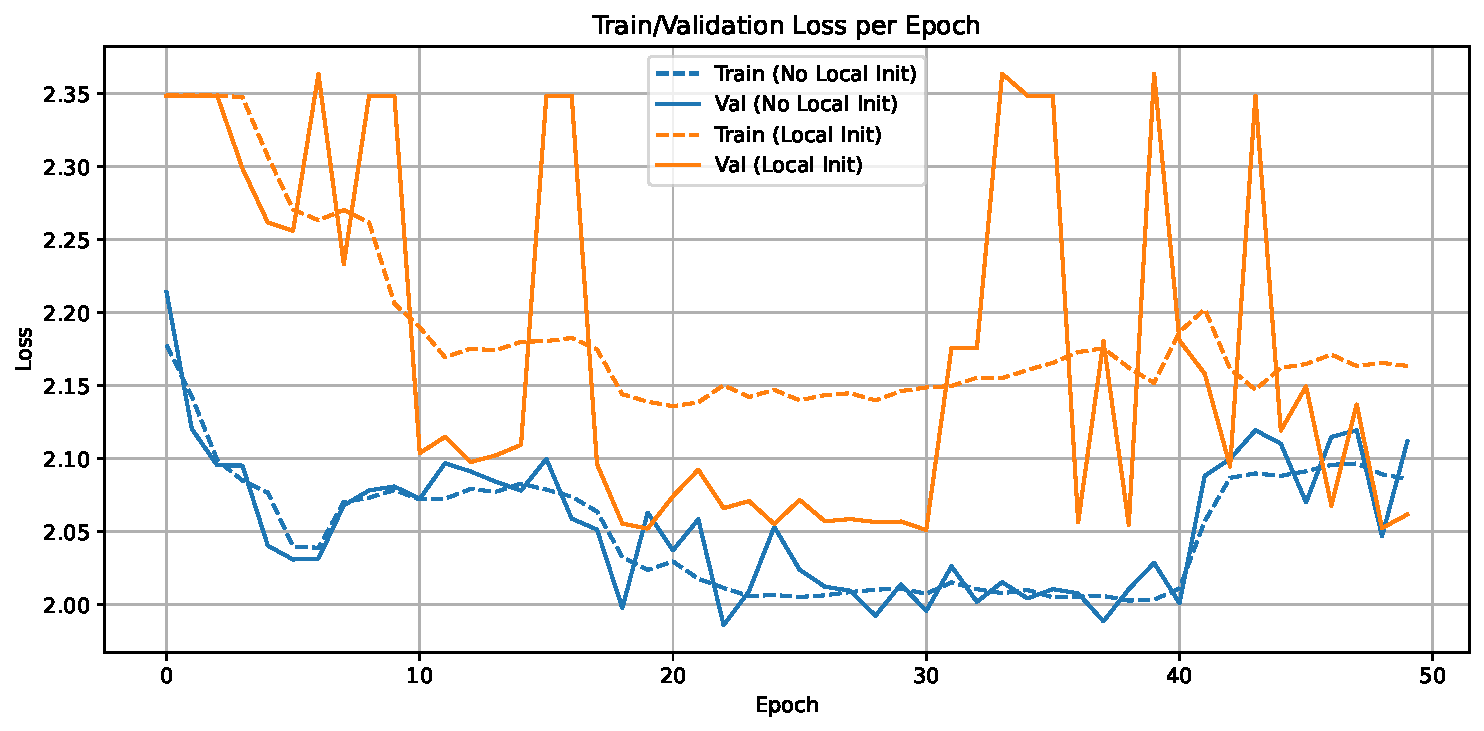
\includegraphics[width=0.45\textwidth]{figures/small_world/loss.pdf}
    \caption{Training and validation accuracy/loss over epochs for OSLGN with and without local operand initialization. Local init generalizes better.}
    \label{fig:smallworld_acc}
\end{figure}

\begin{figure}[H]
    \centering
    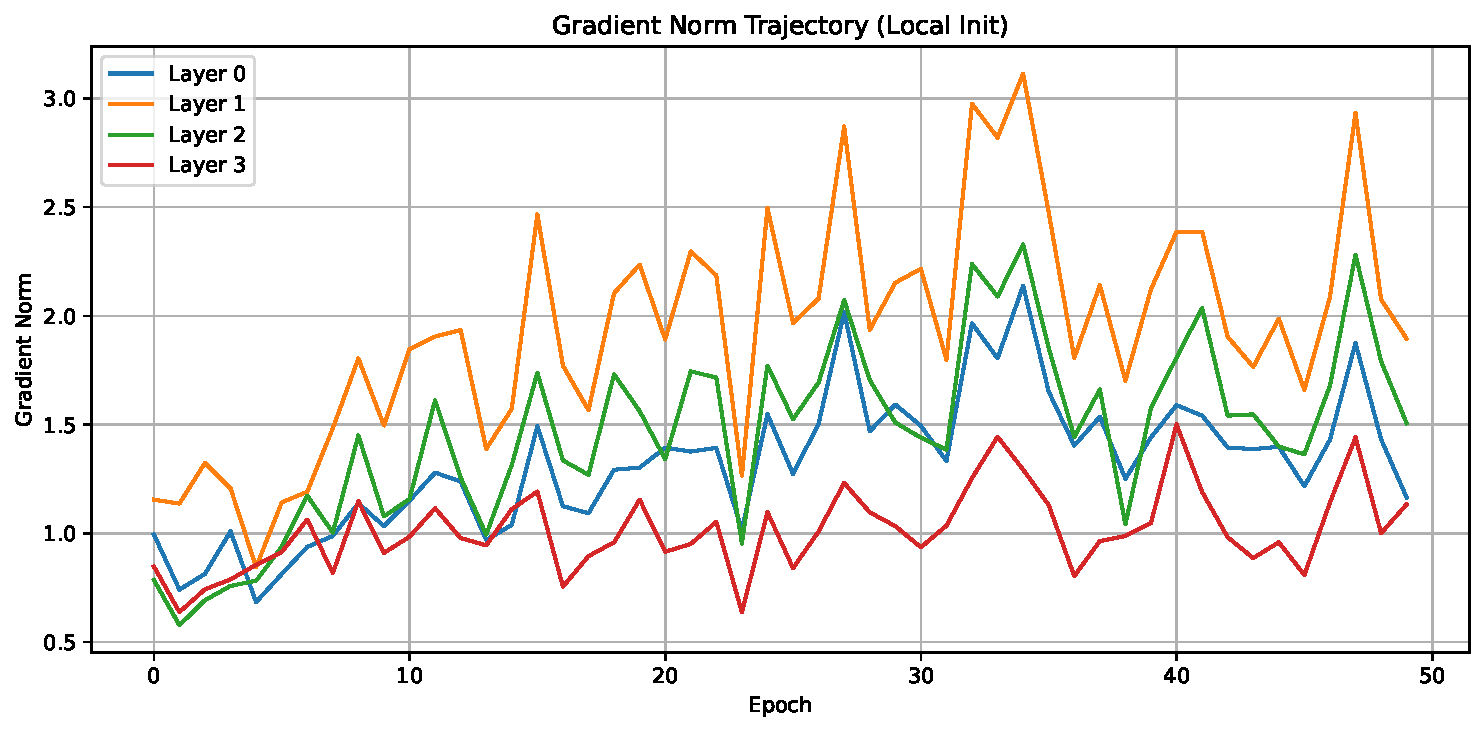
\includegraphics[width=0.85\textwidth]{figures/small_world/gradnorm_lineplot_localinit_on.pdf} \\
    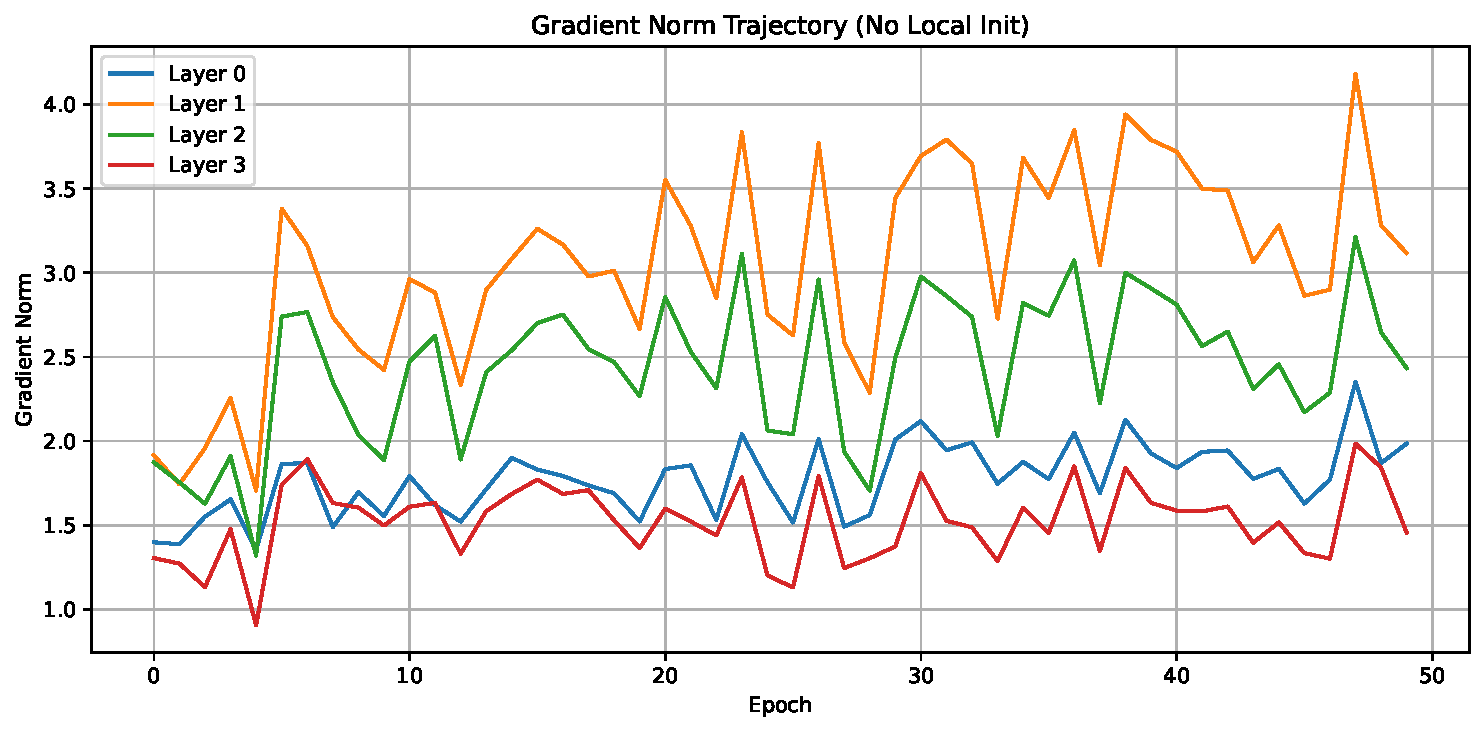
\includegraphics[width=0.85\textwidth]{figures/small_world/gradnorm_lineplot_localinit_off.pdf}
    \caption{Layer-wise gradient norm trajectories with (top) and without (bottom) local operand initialization. Local init results in smoother gradient flow.}
    \label{fig:smallworld_gradnorm}
\end{figure}


\section{Discussion}
  \subsection{Symbolic Structure and Modularity}
    Operand-Selective Logic Gate Networks (OSLGN) construct neural models using symbolic logic gate structures. By selecting operands and logic operators at each layer, OSLGN enables a modular architecture that reflects discrete symbolic computations. Unlike prior approaches that approximate logical rules via fuzzy semantics, our model preserves the syntactic structure of logic circuits throughout training.

  \subsection{Discrete Selection Mechanisms}
    The core mechanism in OSLGN is argmax-based selection with a Straight-Through Estimator (STE), applied to both operand and operator routing. This allows symbolic consistency and gradient-based learning, despite the discrete nature of the computation. While soft selection methods such as Gumbel-Softmax demonstrated faster convergence in preliminary experiments, they require additional stabilization strategies. Future work may explore advanced routing mechanisms to improve convergence speed and training stability.

  \subsection{Topology-Inspired Initialization}
    Inspired by the information flow properties of small-world networks~\cite{watts1998collective, javaheripi2019swnet}, we initialize operand selectors using Gaussian-weighted connectivity centered on local input indices. While not a true small-world topology, this bias promotes modular selection patterns and improves convergence speed, as demonstrated in Section~\ref{sec:experiments}. This structural prior reflects local coherence and allows long-range dependencies to emerge during learning.

  \subsection{Limitations}
    OSLGN currently supports only binary logic gates with hard operand selection. This restricts expressivity in tasks requiring multi-bit reasoning or smooth composition. Additionally, the operand selection layers may introduce redundancy: the learned symbolic expressions often use only a subset of the full network’s capacity, suggesting overparameterization. Another challenge is training stability during early stages, particularly when the routing distributions are uncertain. While softmax-based selection is viable, convergence strategies for stable symbolic gating remain underexplored.

  \subsection{Future Work}
    Future directions include incorporating structured routing techniques and annealing strategies, extending the model to multi-valued or temporal logic, and enabling end-to-end symbolic compression during training. Applying the framework to tasks such as program synthesis, structured decision making, or formal verification remains a promising avenue.


\section{Conclusion}
  Operand-Selective Logic Gate Networks (OSLGN) represent a step toward unifying deep learning with symbolic reasoning. By learning networks of logic gates through operand and operator selection, OSLGN performs symbolic computation while remaining trainable via gradient-based optimization using the Straight-Through Estimator (STE). We showed that this architecture can be initialized with inductive priors to enhance convergence, trained with discrete routing, and post-hoc translated into compact Boolean expressions.

While classification performance remains limited, the symbolic structure of OSLGN supports modularity and compatibility with digital logic. A key challenge is the relatively large network size required to express symbolic patterns, indicating redundancy or inefficiency in operand routing. Our work lays the groundwork for trainable logic circuits and opens the door for future models that are both compact and symbolic, enabling structured and efficient AI systems.


\bibliographystyle{plain}
\bibliography{references}

\appendix
\section{OSLGN Model Implementation}
  \label{appendix:model-code}

The following PyTorch code defines the core components of the Operand Selective Logic Gated Neural Network (OSLGN) model.  
Operand selection uses binary masking via $\arg\max$ with a straight-through estimator (STE), and the operator module composes logic gates among 16 predefined binary functions.  
All logic outputs are strictly binary-valued and verified via runtime assertions.


The logic operator routing and the definition of 16 binary logic gates used in the \texttt{Operator} module are adapted from Petersen et al.~\cite{petersen2022deep}.  
Their original implementation is available at \url{https://github.com/Felix-Petersen/difflogic}.  
Unlike their soft-selection approach, we apply a straight-through estimator (STE) to enforce discrete operator selection during training, enabling train-time quantization within the logic gate routing mechanism.

\subsection{Operand Selector and Logic Operators}

\begin{lstlisting}[language=Python, caption={Operand selection and logic gate definitions.}]
class Operand_selector(nn.Module):
    def __init__(self, x, y):
        super().__init__()
        self.p = nn.Linear(x, y, bias=False)

    def forward(self, x):
        w = self.p.weight
        mask = torch.zeros_like(w).scatter_(1, w.argmax(dim=-1, keepdim=True), 1.0)
        masked = mask - w.detach() + w
        return F.linear(x, masked)
\end{lstlisting}

\subsection{Operator and Logic Layer Composition}
\begin{lstlisting}[language=Python, caption={Operator routing and composition of logic layers.}]
def bin_op(a, b, i):
    if i == 0: return torch.zeros_like(a)
    elif i == 1: return a * b
    elif i == 2: return a - a * b
    elif i == 3: return a
    elif i == 4: return b - a * b
    elif i == 5: return b
    elif i == 6: return a + b - 2 * a * b
    elif i == 7: return a + b - a * b
    elif i == 8: return 1 - (a + b - a * b)
    elif i == 9: return 1 - (a + b - 2 * a * b)
    elif i == 10: return 1 - b
    elif i == 11: return 1 - b + a * b
    elif i == 12: return 1 - a
    elif i == 13: return 1 - a + a * b
    elif i == 14: return 1 - a * b
    elif i == 15: return torch.ones_like(a)


class RoundSTE(torch.autograd.Function):
    @staticmethod
    def forward(ctx, input):
        return torch.round(input)
    @staticmethod
    def backward(ctx, grad_output):
        return grad_output

def bin_op_s(a, b, i_s):
    r = torch.zeros_like(a)
    for i in range(16):
        r += i_s[..., i] * bin_op(a, b, i)
    return RoundSTE.apply(r)

class Operator(nn.Module):
    def __init__(self, y):
        super().__init__()
        self.weights = nn.Parameter(torch.randn(y, 16))

    def forward(self, a, b):
        w = self.weights
        mask = torch.zeros_like(w).scatter_(1, w.argmax(dim=-1, keepdim=True), 1.0)
        masked = mask - w.detach() + w
        return bin_op_s(a, b, masked)

class oslgn(nn.Module):
    def __init__(self, x, y):
        super().__init__()
        self.os1 = Operand_selector(x, y)
        self.os2 = Operand_selector(x, y)
        self.op = Operator(y)

    def forward(self, x):
        a = self.os1(x)
        b = self.os2(x)
        return self.op(a, b)
\end{lstlisting}

\section{Depth Scaling Summary Table}
  To complement the figures in Section~\ref{subsec:Depth Scaling}, Table~\ref{tab:depth_summary} presents a summary of performance metrics for each evaluated depth. 
We report the final and peak validation accuracy across 50 training epochs, along with final validation loss and training accuracy. 
This helps assess both convergence stability and generalization behavior. 
Notably, while depth-4 exhibits both high final and peak accuracy, deeper networks like depth-8 show a wider gap between final and peak accuracy, indicating slower convergence or slight overfitting.

\begin{table}[H]
\centering
\caption{Final and maximum validation accuracy, validation loss, and training accuracy for each depth after 50 epochs.}
\label{tab:depth_summary}
\begin{tabular}{rlll}
\toprule
 Depth &                  Val Acc & Val Loss & Train Acc \\
\midrule
     2 & \textbf{0.4492} / 0.5232 &   1.7693 &    0.4272 \\
     4 & \textbf{0.5330} / 0.5802 &   1.7815 &    0.5073 \\
     8 & \textbf{0.5357} / 0.5958 &   1.7304 &    0.5354 \\
\bottomrule
\end{tabular}
\end{table}

\section{Symbolic Compression of Learned Logic Circuits}
  \label{appendix:symbolic}

The symbolic logic expressions for each output class were derived from the trained OSLGN model (depth=4, 10 epochs). Each expression was reconstructed by backtracking the operand/operator paths through each logic layer. The code implementation is fully available at:

\begin{quote}
\url{https://colab.research.google.com/drive/1VxulftRzLRj1Yg6C-vhmfE6X5jJpxfwJ}
\end{quote}

The original expressions from the model and their compressed forms are presented below.

The symbolic logic expressions for each output class were derived from the trained OSLGN model (depth=4, 10 epochs). Each expression was reconstructed by backtracking the operand/operator paths through each logic layer. The expressions are presented below.

\subsection{Class-wise Boolean Expressions}

\begin{verbatim}
[Class 0]

Original
((((not (x[462] or x[407]) and (x[482] or x[484]))) and 
not ((False) and not ((x[578] or not x[363]) or not (x[107])))) or (False))

Compressed
((not x[462] and not x[407] and x[482]) or (not x[462] and 
not x[407] and x[484]))


[Class 1]
Original   
((((not (x[355] or x[494])) and not (x[261] or x[438])) and not 
(((x[177] and not x[290]) or (False)) or ((x[347] and not x[234]) or (False)))))

Compressed 
((not x[355] and not x[494] and not x[261] and not x[438] and 
x[290] and x[234]) or (not x[355] and not x[494] and not x[261] and not 
x[438] and not x[177] and x[234]) or (not x[355] and not x[494] and not 
x[261] and not x[438] and not x[177] and not x[347]) or (not x[355] and not 
x[494] and not x[261] and not x[438] and x[290] and not x[347]))

[Class 2]
Original
((((not x[372] and x[541]) and not (x[347] and not x[556]))) or 
((not (x[319] or x[276])) and ((not x[343] and x[511]))))

Compressed
((not x[372] and x[541] and x[556]) or (not x[319] and not x[276] and not 
x[343] and x[511]) or (not x[347] and not x[372] and x[541]))

[Class 3]
Original
(not (not (((x[350] or x[322]) and (x[152] or x[179])) or 
((x[649]) or (not x[455] and x[564])))))

Compressed
(x[649] or (x[322] and x[152]) or (x[350] and x[152]) or 
(not x[455] and x[564]) or (x[350] and x[179]) or (x[322] and x[179]))

[Class 4]
Original  
(not (not ((not (((x[211] and not x[68]) or (False)) or 
(x[567] or x[127]))) and ((x[401] or x[429]) and (not (x[70] or x[747]))))) or 
(((not (x[568] or x[595])) and (x[454]))))

Compressed
((x[68] and not x[567] and not x[127] and x[429] and not x[70] and not 
x[747]) or (not x[568] and not x[595] and x[454]) or (x[68] and not 
x[567] and not x[127] and x[401] and not x[70] and not x[747]) or 
(not x[211] and not x[567] and not x[127] and x[401] and not x[70] and not 
x[747]) or (not x[211] and not x[567] and not x[127] and x[429] and not 
x[70] and not x[747]))

[Class 5]
Original
(not (((not x[562] and x[517]) and (not x[562] and x[517])) and 
((not x[562] and x[517]) and (not x[562] and x[517]))) and 
(not ((x[246]) and (x[356] and not x[587])) and (not (x[355]) and 
((x[191] and not x[276]) or (False)))))

Compressed
((not x[355] and not x[276] and not x[517] and x[587] and x[191]) or 
(not x[355] and not x[276] and x[562] and not x[356] and x[191]) or 
(not x[355] and not x[276] and x[562] and x[587] and x[191]) or 
(not x[355] and not x[276] and x[562] and not x[246] and x[191]) or 
(not x[355] and not x[276] and not x[517] and not x[356] and x[191]) or 
(not x[355] and not x[276] and not x[517] and not x[246] and x[191]))

[Class 6]
Original
(not ((((x[651] or x[658]))) and (((x[651] or x[658])))))

Compressed
(not x[651] and not x[658])

[Class 7]
Original
((((not (x[377] or x[404])))))

Compressed
(not x[377] and not x[404])

[Class 8]
Original   
(True)

Compressed 
(not x[377] and not x[404])

[Class 9]
Original
(not ((((x[149] and not x[127]) and not (x[567] or x[127])) or (False)) and 
not ((x[714] and not x[203]))) or ((((x[149] and not x[127]) and 
not (x[396] or not x[126])) or (False)) and ((not x[567] and x[711]))))

Compressed
(x[567] or x[127] or not x[149] or (x[714] and not x[203]) or 
(not x[396] and x[126] and x[711]))

\end{verbatim}
\subsection{Compression Results}

\begin{table}[H]
    \caption{Comparison of logic operator counts before and after symbolic compression using PyEDA.}
    \label{tab:symbolic_compression}
    \centering
    \small
    \begin{tabular}{c|cccc}
        \toprule
        \textbf{Class} & \textbf{Original Ops} & \textbf{Compressed Ops} & \textbf{Ratio} & \textbf{Rate (\%)} \\
        \midrule
        0 & 13 & 9 & 1.44 & 30.77 \\
        1 & 14 & 43 & 0.33 & -207.14 \\
        2 & 12 & 15 & 0.8 & -25 \\
        3 & 9 & 11 & 0.82 & -22.22 \\
        4 & 17 & 46 & 0.37 & -170.59 \\
        5 & 23 & 48 & 0.48 & -108.7 \\
        6 & 18 & 62 & 0.29 & -244.4 \\
        7 & 2 & 3 & 0.67 & -50 \\
        8 & 0 & 3 & 0 & 0 \\
        9 & 22 & 10 & 2.2 & 54.55 \\
        \bottomrule
    \end{tabular}

\end{table}

\noindent These results confirm that OSLGN produces structurally compact logic by design, rather than relying on post-hoc symbolic simplification.


\newpage
\section*{NeurIPS Paper Checklist}
  % %%% BEGIN INSTRUCTIONS %%%
% The checklist is designed to encourage best practices for responsible machine learning research, addressing issues of reproducibility, transparency, research ethics, and societal impact. Do not remove the checklist: {\bf The papers not including the checklist will be desk rejected.} The checklist should follow the references and follow the (optional) supplemental material.  The checklist does NOT count towards the page
% limit. 

% Please read the checklist guidelines carefully for information on how to answer these questions. For each question in the checklist:
% \begin{itemize}
%     \item You should answer \answerYes{}, \answerNo{}, or \answerNA{}.
%     \item \answerNA{} means either that the question is Not Applicable for that particular paper or the relevant information is Not Available.
%     \item Please provide a short (1–2 sentence) justification right after your answer (even for NA). 
%    % \item {\bf The papers not including the checklist will be desk rejected.}
% \end{itemize}

% {\bf The checklist answers are an integral part of your paper submission.} They are visible to the reviewers, area chairs, senior area chairs, and ethics reviewers. You will be asked to also include it (after eventual revisions) with the final version of your paper, and its final version will be published with the paper.

% The reviewers of your paper will be asked to use the checklist as one of the factors in their evaluation. While "\answerYes{}" is generally preferable to "\answerNo{}", it is perfectly acceptable to answer "\answerNo{}" provided a proper justification is given (e.g., "error bars are not reported because it would be too computationally expensive" or "we were unable to find the license for the dataset we used"). In general, answering "\answerNo{}" or "\answerNA{}" is not grounds for rejection. While the questions are phrased in a binary way, we acknowledge that the true answer is often more nuanced, so please just use your best judgment and write a justification to elaborate. All supporting evidence can appear either in the main paper or the supplemental material, provided in appendix. If you answer \answerYes{} to a question, in the justification please point to the section(s) where related material for the question can be found.

% IMPORTANT, please:
% \begin{itemize}
%     \item {\bf Delete this instruction block, but keep the section heading ``NeurIPS Paper Checklist"},
%     \item  {\bf Keep the checklist subsection headings, questions/answers and guidelines below.}
%     \item {\bf Do not modify the questions and only use the provided macros for your answers}.
% \end{itemize} 
 

% %%% END INSTRUCTIONS %%%


\begin{enumerate}

\item {\bf Claims}
    \item[] Question: Do the main claims made in the abstract and introduction accurately reflect the paper's contributions and scope?
    \item[] Answer: \answerYes{} % Replace by \answerYes{}, \answerNo{}, or \answerNA{}.
    \item[] Justification: Since the research is originally to show our method can be learned, it is shown through experiment results and the codes we appended.
    \item[] Guidelines:
    \begin{itemize}
        \item The answer NA means that the abstract and introduction do not include the claims made in the paper.
        \item The abstract and/or introduction should clearly state the claims made, including the contributions made in the paper and important assumptions and limitations. A No or NA answer to this question will not be perceived well by the reviewers. 
        \item The claims made should match theoretical and experimental results, and reflect how much the results can be expected to generalize to other settings. 
        \item It is fine to include aspirational goals as motivation as long as it is clear that these goals are not attained by the paper. 
    \end{itemize}

\item {\bf Limitations}
    \item[] Question: Does the paper discuss the limitations of the work performed by the authors?
    \item[] Answer: \answerYes{} % Replace by \answerYes{}, \answerNo{}, or \answerNA{}.
    \item[] Justification: Since this model is conceptually new, intended to avoid tricks like normalization, and can be result in extremely compact expression, its accuracy is yet relatively low. However, its modularity would be effective feature when it is studied further.
    \item[] Guidelines:
    \begin{itemize}
        \item The answer NA means that the paper has no limitation while the answer No means that the paper has limitations, but those are not discussed in the paper. 
        \item The authors are encouraged to create a separate "Limitations" section in their paper.
        \item The paper should point out any strong assumptions and how robust the results are to violations of these assumptions (e.g., independence assumptions, noiseless settings, model well-specification, asymptotic approximations only holding locally). The authors should reflect on how these assumptions might be violated in practice and what the implications would be.
        \item The authors should reflect on the scope of the claims made, e.g., if the approach was only tested on a few datasets or with a few runs. In general, empirical results often depend on implicit assumptions, which should be articulated.
        \item The authors should reflect on the factors that influence the performance of the approach. For example, a facial recognition algorithm may perform poorly when image resolution is low or images are taken in low lighting. Or a speech-to-text system might not be used reliably to provide closed captions for online lectures because it fails to handle technical jargon.
        \item The authors should discuss the computational efficiency of the proposed algorithms and how they scale with dataset size.
        \item If applicable, the authors should discuss possible limitations of their approach to address problems of privacy and fairness.
        \item While the authors might fear that complete honesty about limitations might be used by reviewers as grounds for rejection, a worse outcome might be that reviewers discover limitations that aren't acknowledged in the paper. The authors should use their best judgment and recognize that individual actions in favor of transparency play an important role in developing norms that preserve the integrity of the community. Reviewers will be specifically instructed to not penalize honesty concerning limitations.
    \end{itemize}

\item {\bf Theory assumptions and proofs}
    \item[] Question: For each theoretical result, does the paper provide the full set of assumptions and a complete (and correct) proof?
    \item[] Answer: \answerNA{} % Replace by \answerYes{}, \answerNo{}, or \answerNA{}.
    \item[] Justification: The research is more about extending and combining existing theories. We chose to show its effectiveness with experiments.
    \item[] Guidelines:
    \begin{itemize}
        \item The answer NA means that the paper does not include theoretical results. 
        \item All the theorems, formulas, and proofs in the paper should be numbered and cross-referenced.
        \item All assumptions should be clearly stated or referenced in the statement of any theorems.
        \item The proofs can either appear in the main paper or the supplemental material, but if they appear in the supplemental material, the authors are encouraged to provide a short proof sketch to provide intuition. 
        \item Inversely, any informal proof provided in the core of the paper should be complemented by formal proofs provided in appendix or supplemental material.
        \item Theorems and Lemmas that the proof relies upon should be properly referenced. 
    \end{itemize}

    \item {\bf Experimental result reproducibility}
    \item[] Question: Does the paper fully disclose all the information needed to reproduce the main experimental results of the paper to the extent that it affects the main claims and/or conclusions of the paper (regardless of whether the code and data are provided or not)?
    \item[] Answer: \answerYes{} % Replace by \answerYes{}, \answerNo{}, or \answerNA{}.
    \item[] Justification: Every code used in this paper are served with google colab link. And the python code is appended for structural reproduction.
    \item[] Guidelines:
    \begin{itemize}
        \item The answer NA means that the paper does not include experiments.
        \item If the paper includes experiments, a No answer to this question will not be perceived well by the reviewers: Making the paper reproducible is important, regardless of whether the code and data are provided or not.
        \item If the contribution is a dataset and/or model, the authors should describe the steps taken to make their results reproducible or verifiable. 
        \item Depending on the contribution, reproducibility can be accomplished in various ways. For example, if the contribution is a novel architecture, describing the architecture fully might suffice, or if the contribution is a specific model and empirical evaluation, it may be necessary to either make it possible for others to replicate the model with the same dataset, or provide access to the model. In general. releasing code and data is often one good way to accomplish this, but reproducibility can also be provided via detailed instructions for how to replicate the results, access to a hosted model (e.g., in the case of a large language model), releasing of a model checkpoint, or other means that are appropriate to the research performed.
        \item While NeurIPS does not require releasing code, the conference does require all submissions to provide some reasonable avenue for reproducibility, which may depend on the nature of the contribution. For example
        \begin{enumerate}
            \item If the contribution is primarily a new algorithm, the paper should make it clear how to reproduce that algorithm.
            \item If the contribution is primarily a new model architecture, the paper should describe the architecture clearly and fully.
            \item If the contribution is a new model (e.g., a large language model), then there should either be a way to access this model for reproducing the results or a way to reproduce the model (e.g., with an open-source dataset or instructions for how to construct the dataset).
            \item We recognize that reproducibility may be tricky in some cases, in which case authors are welcome to describe the particular way they provide for reproducibility. In the case of closed-source models, it may be that access to the model is limited in some way (e.g., to registered users), but it should be possible for other researchers to have some path to reproducing or verifying the results.
        \end{enumerate}
    \end{itemize}


\item {\bf Open access to data and code}
    \item[] Question: Does the paper provide open access to the data and code, with sufficient instructions to faithfully reproduce the main experimental results, as described in supplemental material?
    \item[] Answer: \answerYes{} % Replace by \answerYes{}, \answerNo{}, or \answerNA{}.
    \item[] Justification: It is all given as above. Dataset we used is benchmark dataset and the code to retrieve is already served.
    \item[] Guidelines:
    \begin{itemize}
        \item The answer NA means that paper does not include experiments requiring code.
        \item Please see the NeurIPS code and data submission guidelines (\url{https://nips.cc/public/guides/CodeSubmissionPolicy}) for more details.
        \item While we encourage the release of code and data, we understand that this might not be possible, so “No” is an acceptable answer. Papers cannot be rejected simply for not including code, unless this is central to the contribution (e.g., for a new open-source benchmark).
        \item The instructions should contain the exact command and environment needed to run to reproduce the results. See the NeurIPS code and data submission guidelines (\url{https://nips.cc/public/guides/CodeSubmissionPolicy}) for more details.
        \item The authors should provide instructions on data access and preparation, including how to access the raw data, preprocessed data, intermediate data, and generated data, etc.
        \item The authors should provide scripts to reproduce all experimental results for the new proposed method and baselines. If only a subset of experiments are reproducible, they should state which ones are omitted from the script and why.
        \item At submission time, to preserve anonymity, the authors should release anonymized versions (if applicable).
        \item Providing as much information as possible in supplemental material (appended to the paper) is recommended, but including URLs to data and code is permitted.
    \end{itemize}


\item {\bf Experimental setting/details}
    \item[] Question: Does the paper specify all the training and test details (e.g., data splits, hyperparameters, how they were chosen, type of optimizer, etc.) necessary to understand the results?
    \item[] Answer: \answerYes{} % Replace by \answerYes{}, \answerNo{}, or \answerNA{}.
    \item[] Justification: In the paper there are critical settings you should know, and in the code you are able to get exact environment.
    \item[] Guidelines:
    \begin{itemize}
        \item The answer NA means that the paper does not include experiments.
        \item The experimental setting should be presented in the core of the paper to a level of detail that is necessary to appreciate the results and make sense of them.
        \item The full details can be provided either with the code, in appendix, or as supplemental material.
    \end{itemize}

\item {\bf Experiment statistical significance}
    \item[] Question: Does the paper report error bars suitably and correctly defined or other appropriate information about the statistical significance of the experiments?
    \item[] Answer: \answerNo{} % Replace by \answerYes{}, \answerNo{}, or \answerNA{}.
    \item[] Justification: However, the experiment is very well known mnist and the exact method is available through served colab link.
    \item[] Guidelines:
    \begin{itemize}
        \item The answer NA means that the paper does not include experiments.
        \item The authors should answer "Yes" if the results are accompanied by error bars, confidence intervals, or statistical significance tests, at least for the experiments that support the main claims of the paper.
        \item The factors of variability that the error bars are capturing should be clearly stated (for example, train/test split, initialization, random drawing of some parameter, or overall run with given experimental conditions).
        \item The method for calculating the error bars should be explained (closed form formula, call to a library function, bootstrap, etc.)
        \item The assumptions made should be given (e.g., Normally distributed errors).
        \item It should be clear whether the error bar is the standard deviation or the standard error of the mean.
        \item It is OK to report 1-sigma error bars, but one should state it. The authors should preferably report a 2-sigma error bar than state that they have a 96\% CI, if the hypothesis of Normality of errors is not verified.
        \item For asymmetric distributions, the authors should be careful not to show in tables or figures symmetric error bars that would yield results that are out of range (e.g. negative error rates).
        \item If error bars are reported in tables or plots, The authors should explain in the text how they were calculated and reference the corresponding figures or tables in the text.
    \end{itemize}

\item {\bf Experiments compute resources}
    \item[] Question: For each experiment, does the paper provide sufficient information on the computer resources (type of compute workers, memory, time of execution) needed to reproduce the experiments?
    \item[] Answer: \answerYes{} % Replace by \answerYes{}, \answerNo{}, or \answerNA{}.
    \item[] Justification: Experiment was performed through google colab and it is mentioned.
    \item[] Guidelines:
    \begin{itemize}
        \item The answer NA means that the paper does not include experiments.
        \item The paper should indicate the type of compute workers CPU or GPU, internal cluster, or cloud provider, including relevant memory and storage.
        \item The paper should provide the amount of compute required for each of the individual experimental runs as well as estimate the total compute. 
        \item The paper should disclose whether the full research project required more compute than the experiments reported in the paper (e.g., preliminary or failed experiments that didn't make it into the paper). 
    \end{itemize}
    
\item {\bf Code of ethics}
    \item[] Question: Does the research conducted in the paper conform, in every respect, with the NeurIPS Code of Ethics \url{https://neurips.cc/public/EthicsGuidelines}?
    \item[] Answer: \answerNA{} % Replace by \answerYes{}, \answerNo{}, or \answerNA{}.
    \item[] Justification: The paper focuses on a foundational architecture, with no direct deployment or societal interface. As such, it does not raise immediate social impact concerns.

    \item[] Guidelines:
    \begin{itemize}
        \item The answer NA means that the authors have not reviewed the NeurIPS Code of Ethics.
        \item If the authors answer No, they should explain the special circumstances that require a deviation from the Code of Ethics.
        \item The authors should make sure to preserve anonymity (e.g., if there is a special consideration due to laws or regulations in their jurisdiction).
    \end{itemize}


\item {\bf Broader impacts}
    \item[] Question: Does the paper discuss both potential positive societal impacts and negative societal impacts of the work performed?
    \item[] Answer: \answerYes{} % Replace by \answerYes{}, \answerNo{}, or \answerNA{}.
    \item[] Justification: While our work is primarily foundational, symbolic reasoning systems could enable more controllable AI in sensitive domains. We acknowledge the potential for misuse in automation of decision logic and advocate for responsible deployment.
    \item[] Guidelines:
    \begin{itemize}
        \item The answer NA means that there is no societal impact of the work performed.
        \item If the authors answer NA or No, they should explain why their work has no societal impact or why the paper does not address societal impact.
        \item Examples of negative societal impacts include potential malicious or unintended uses (e.g., disinformation, generating fake profiles, surveillance), fairness considerations (e.g., deployment of technologies that could make decisions that unfairly impact specific groups), privacy considerations, and security considerations.
        \item The conference expects that many papers will be foundational research and not tied to particular applications, let alone deployments. However, if there is a direct path to any negative applications, the authors should point it out. For example, it is legitimate to point out that an improvement in the quality of generative models could be used to generate deepfakes for disinformation. On the other hand, it is not needed to point out that a generic algorithm for optimizing neural networks could enable people to train models that generate Deepfakes faster.
        \item The authors should consider possible harms that could arise when the technology is being used as intended and functioning correctly, harms that could arise when the technology is being used as intended but gives incorrect results, and harms following from (intentional or unintentional) misuse of the technology.
        \item If there are negative societal impacts, the authors could also discuss possible mitigation strategies (e.g., gated release of models, providing defenses in addition to attacks, mechanisms for monitoring misuse, mechanisms to monitor how a system learns from feedback over time, improving the efficiency and accessibility of ML).
    \end{itemize}
    
\item {\bf Safeguards}
    \item[] Question: Does the paper describe safeguards that have been put in place for responsible release of data or models that have a high risk for misuse (e.g., pretrained language models, image generators, or scraped datasets)?
    \item[] Answer: \answerNA{} % Replace by \answerYes{}, \answerNo{}, or \answerNA{}.
    \item[] Justification: No deployable models or data are released; the work is conceptual.
    \item[] Guidelines:
    \begin{itemize}
        \item The answer NA means that the paper poses no such risks.
        \item Released models that have a high risk for misuse or dual-use should be released with necessary safeguards to allow for controlled use of the model, for example by requiring that users adhere to usage guidelines or restrictions to access the model or implementing safety filters. 
        \item Datasets that have been scraped from the Internet could pose safety risks. The authors should describe how they avoided releasing unsafe images.
        \item We recognize that providing effective safeguards is challenging, and many papers do not require this, but we encourage authors to take this into account and make a best faith effort.
    \end{itemize}

\item {\bf Licenses for existing assets}
    \item[] Question: Are the creators or original owners of assets (e.g., code, data, models), used in the paper, properly credited and are the license and terms of use explicitly mentioned and properly respected?
    \item[] Answer: \answerYes{} % Replace by \answerYes{}, \answerNo{}, or \answerNA{}.
    \item[] Justification: Yes.
    \item[] Guidelines:
    \begin{itemize}
        \item The answer NA means that the paper does not use existing assets.
        \item The authors should cite the original paper that produced the code package or dataset.
        \item The authors should state which version of the asset is used and, if possible, include a URL.
        \item The name of the license (e.g., CC-BY 4.0) should be included for each asset.
        \item For scraped data from a particular source (e.g., website), the copyright and terms of service of that source should be provided.
        \item If assets are released, the license, copyright information, and terms of use in the package should be provided. For popular datasets, \url{paperswithcode.com/datasets} has curated licenses for some datasets. Their licensing guide can help determine the license of a dataset.
        \item For existing datasets that are re-packaged, both the original license and the license of the derived asset (if it has changed) should be provided.
        \item If this information is not available online, the authors are encouraged to reach out to the asset's creators.
    \end{itemize}

\item {\bf New assets}
    \item[] Question: Are new assets introduced in the paper well documented and is the documentation provided alongside the assets?
    \item[] Answer: \answerNA{} % Replace by \answerYes{}, \answerNo{}, or \answerNA{}.
    \item[] Justification: No new assets. However git and pip could be distributed if there are demands.
    \item[] Guidelines:
    \begin{itemize}
        \item The answer NA means that the paper does not release new assets.
        \item Researchers should communicate the details of the dataset/code/model as part of their submissions via structured templates. This includes details about training, license, limitations, etc. 
        \item The paper should discuss whether and how consent was obtained from people whose asset is used.
        \item At submission time, remember to anonymize your assets (if applicable). You can either create an anonymized URL or include an anonymized zip file.
    \end{itemize}

\item {\bf Crowdsourcing and research with human subjects}
    \item[] Question: For crowdsourcing experiments and research with human subjects, does the paper include the full text of instructions given to participants and screenshots, if applicable, as well as details about compensation (if any)? 
    \item[] Answer: \answerNA{} % Replace by \answerYes{}, \answerNo{}, or \answerNA{}.
    \item[] Justification: There is possiblility to contact one or two in the future, but not now.
    \item[] Guidelines:
    \begin{itemize}
        \item The answer NA means that the paper does not involve crowdsourcing nor research with human subjects.
        \item Including this information in the supplemental material is fine, but if the main contribution of the paper involves human subjects, then as much detail as possible should be included in the main paper. 
        \item According to the NeurIPS Code of Ethics, workers involved in data collection, curation, or other labor should be paid at least the minimum wage in the country of the data collector. 
    \end{itemize}

\item {\bf Institutional review board (IRB) approvals or equivalent for research with human subjects}
    \item[] Question: Does the paper describe potential risks incurred by study participants, whether such risks were disclosed to the subjects, and whether Institutional Review Board (IRB) approvals (or an equivalent approval/review based on the requirements of your country or institution) were obtained?
    \item[] Answer: \answerNA{} % Replace by \answerYes{}, \answerNo{}, or \answerNA{}.
    \item[] Justification: No chance at all.
    \item[] Guidelines:
    \begin{itemize}
        \item The answer NA means that the paper does not involve crowdsourcing nor research with human subjects.
        \item Depending on the country in which research is conducted, IRB approval (or equivalent) may be required for any human subjects research. If you obtained IRB approval, you should clearly state this in the paper. 
        \item We recognize that the procedures for this may vary significantly between institutions and locations, and we expect authors to adhere to the NeurIPS Code of Ethics and the guidelines for their institution. 
        \item For initial submissions, do not include any information that would break anonymity (if applicable), such as the institution conducting the review.
    \end{itemize}

\item {\bf Declaration of LLM usage}
    \item[] Question: Does the paper describe the usage of LLMs if it is an important, original, or non-standard component of the core methods in this research? Note that if the LLM is used only for writing, editing, or formatting purposes and does not impact the core methodology, scientific rigorousness, or originality of the research, declaration is not required.
    %this research? 
    \item[] Answer: \answerYes{} % Replace by \answerYes{}, \answerNo{}, or \answerNA{}.
    \item[] Justification: ChatGPT helped us a lot for making this work real and be ready to be published.
    \item[] Guidelines:
    \begin{itemize}
        \item The answer NA means that the core method development in this research does not involve LLMs as any important, original, or non-standard components.
        \item Please refer to our LLM policy (\url{https://neurips.cc/Conferences/2025/LLM}) for what should or should not be described.
    \end{itemize}

\end{enumerate}


\end{document}